\documentclass[UTF8,AutoFakeBold,a4paper]{article}
\usepackage{ctex}
\usepackage{framed}
\usepackage{amsthm}
\usepackage{geometry}
\usepackage{amsthm,amsmath,amssymb}
\usepackage{mathrsfs}
\geometry{left=2.5cm,right=2.5cm,top=2.5cm,bottom=2.5cm}
\usepackage{amsmath}
\usepackage{graphicx}
\usepackage{multirow}
\usepackage{subfiles}
\linespread{1.314}
%\usepackage{luatexja-fontspec}
\setCJKmainfont[ItalicFont=FandolKai-Regular,BoldFont=STSongti-SC-Black]{SimSun} 
\usepackage{physics}
\usepackage{graphicx}
\usepackage{arydshln}
\setCJKfamilyfont{kaiti}{FandolKai-Regular}
\newcommand{\kaiti}{\CJKfamily{kaiti}}%
\usepackage{paralist}
\everymath{\displaystyle}
\usepackage{chngcntr}%图片编号的宏包
\counterwithout{figure}{section}%取消图片按章节编号
\counterwithin{figure}{section}%将equation环境重新编号,不按节编号
%\usepackage{emoji}
%\usepackage{ntheorem}
%\setemojifont{Twemoji Mozilla} 
%
%\usepackage{multicol}
%\let\itemize\compactitem
%\let\enditemize\endcompactitem
%\let\enumerate\compactenum
%\let\endenumerate\endcompactenum
%\let\description\compactdesc
%\let\enddescription\endcompactdesc
\usepackage{color}
\usepackage{fancyhdr} %调用宏包

% ---基本设置---

%设定页面的页眉页脚类型,$\LaTeX$内置了四种:empty、plain、headings及myheadings
\pagestyle{fancy}

%清除原页眉页脚样式
\fancyhf{} 

%R:页面右边;O:奇数页;\leftmark:表示“一级标题”
\fancyhead[CO]{\leftmark}

%L:页面左边;E:偶数页;\rightmark:表示“二级标题”
\fancyhead[CE]{\rightmark}

%C:页面中间
\fancyhead[CO, CE]{物理化学实验数据处理}

% 设置页脚,页眉的位置上也可以放置页码
\fancyfoot[CO]{\thepage}

% 设置页眉页脚横线及样式
%页眉线宽,设为0可以去页眉线
\renewcommand{\headrulewidth}{0.5pt} 

\usepackage{listings}

{
\lstset{numbers=left, %设置行号位置
        numberstyle=\zihao{-5}, %设置行号大小
        keywordstyle=\textcolor[rgb]{0.07,0.36,0.57}, %设置关键字颜色
        commentstyle=\textcolor[rgb]{0.21,0.49,0.30}, %设置注释颜色
        escapeinside=``, %逃逸字符(1左面的键),用于显示中文
        extendedchars=false, 
        xleftmargin=2em,xrightmargin=2em, aboveskip=1em, %设置边距
        tabsize=4, %设置tab空格数
        showspaces=false %不显示空格
       }

\title{\textbf{物理化学实验}}
\date{\today}
\author{B.H.Zhang}
%\setmainfont{Times New Roman}
%\setCJKsansfont{STSong}
%%\setCJKmainfont[BoldFont=STHeiti]{STSong}
%%\setCJKmainfont{STXihei}
%\setCJKmonofont{STXihei}
\usepackage{chemfig}
\usepackage{mathrsfs}
\usepackage{listings}
\usepackage{makeidx}
\makeindex
\usepackage{framed}
\usepackage{amsthm,amsmath,amssymb}
\usepackage{wrapfig}
\usepackage{graphicx}
\usepackage{mathrsfs}
\bibliographystyle{plain}
\usepackage{subfiles}
\usepackage{booktabs}
\usepackage{graphicx,times}
\usepackage{esint}
\usepackage{times}
\usepackage{subfigure}         
\usepackage{natbib}
\usepackage{amssymb,amsmath}
\usepackage{url}
\usepackage{geometry}
\usepackage{xcolor}
\usepackage{setspace}
\usepackage{subfigure}
\usepackage{booktabs}
\usepackage{array}
\usepackage{mhchem}
%\usepackage[usenames,dvipsnames]{color}
\usepackage{colortbl}
\usepackage{bm}
\usepackage{calligra}
\definecolor{mygray}{gray}{.9}
\definecolor{mypink}{rgb}{.99,.91,.95}
\definecolor{mycyan}{cmyk}{.3,0,0,0}
\definecolor{myorgn}{rgb}{0.56,0.28,0.16}
\definecolor{myyelo}{rgb}{255,215,0}
\usepackage{environ}
\everymath{\displaystyle}  
\usepackage[breaklinks,colorlinks,linkcolor=black,citecolor=black,urlcolor=black]{hyperref}
\usepackage{tikz}
\begin{document}
	\maketitle
	\section{实验一:燃烧焓的测定}
	\begin{figure}[h]
	\centering
	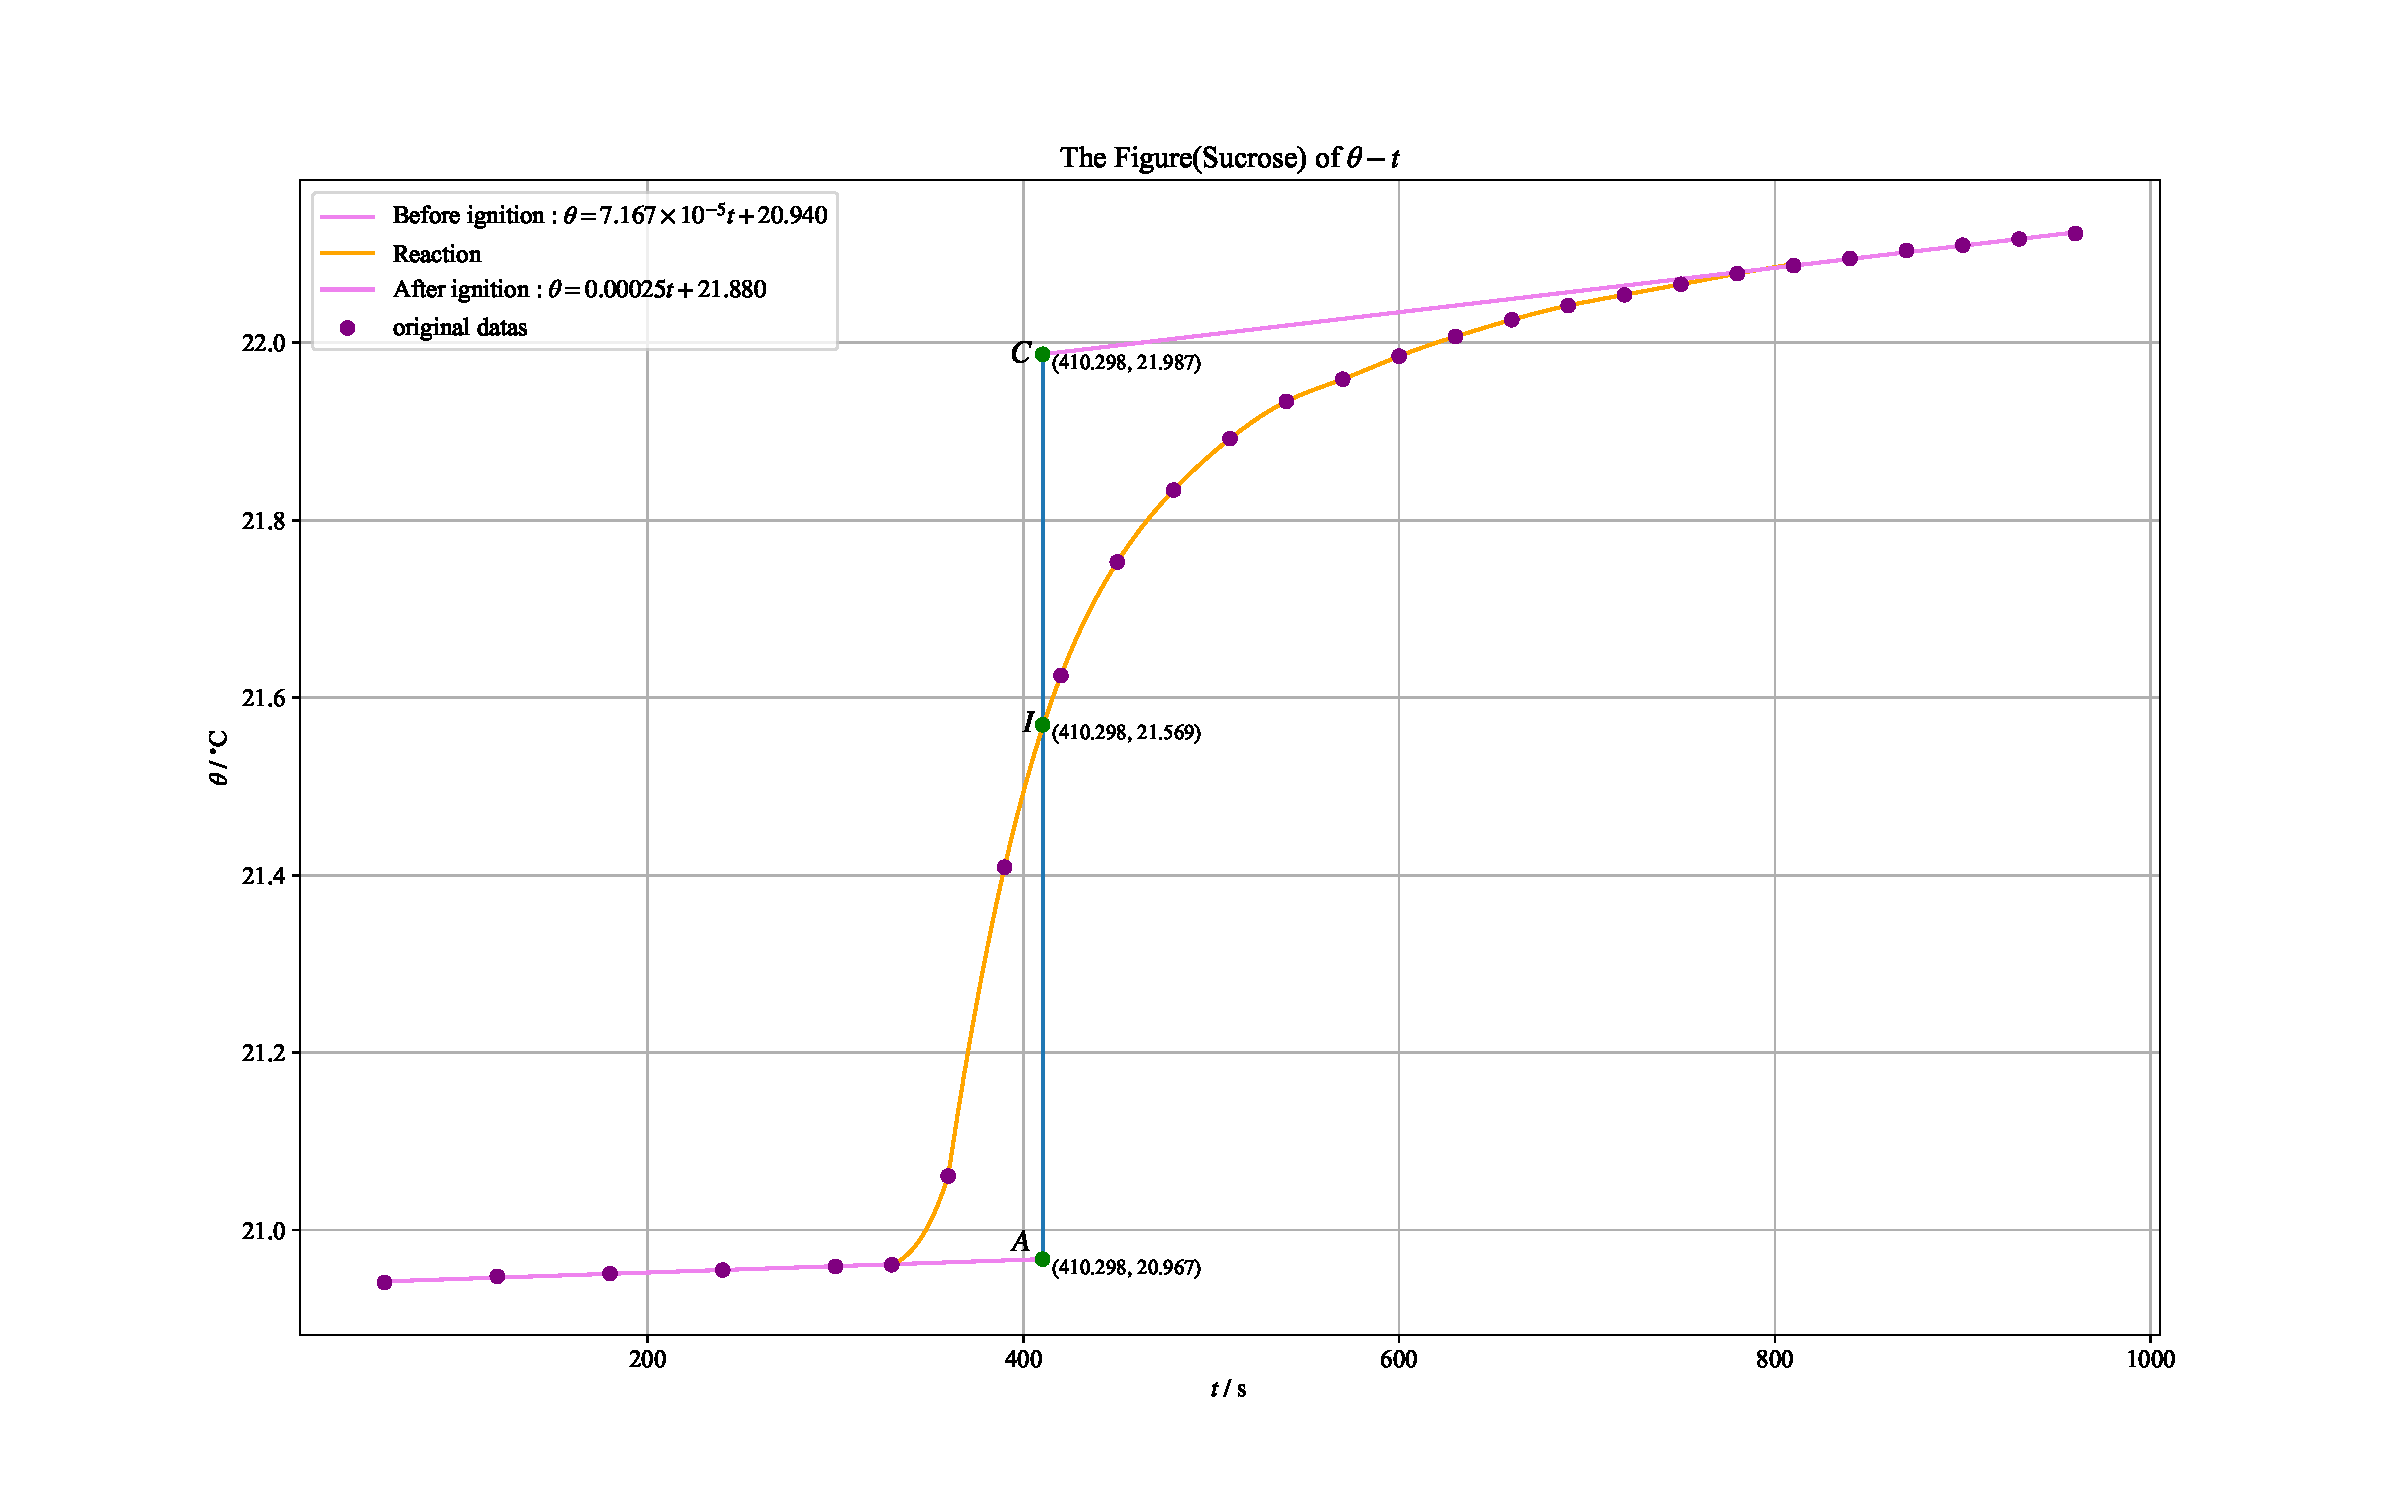
\includegraphics[scale=0.4]{Fig1}
	\caption{蔗糖的雷诺校正曲线。纵坐标$\theta$为温度(去单位为摄氏度$^{\circ}$C),横坐标$t$为时间(去单位为 秒 s),$C$点与$A$点纵坐标差值为升高温度为$1.020^{\circ}$C}
	\label{fi6}
\end{figure}
\newpage
	\begin{figure}[h]
	\centering
	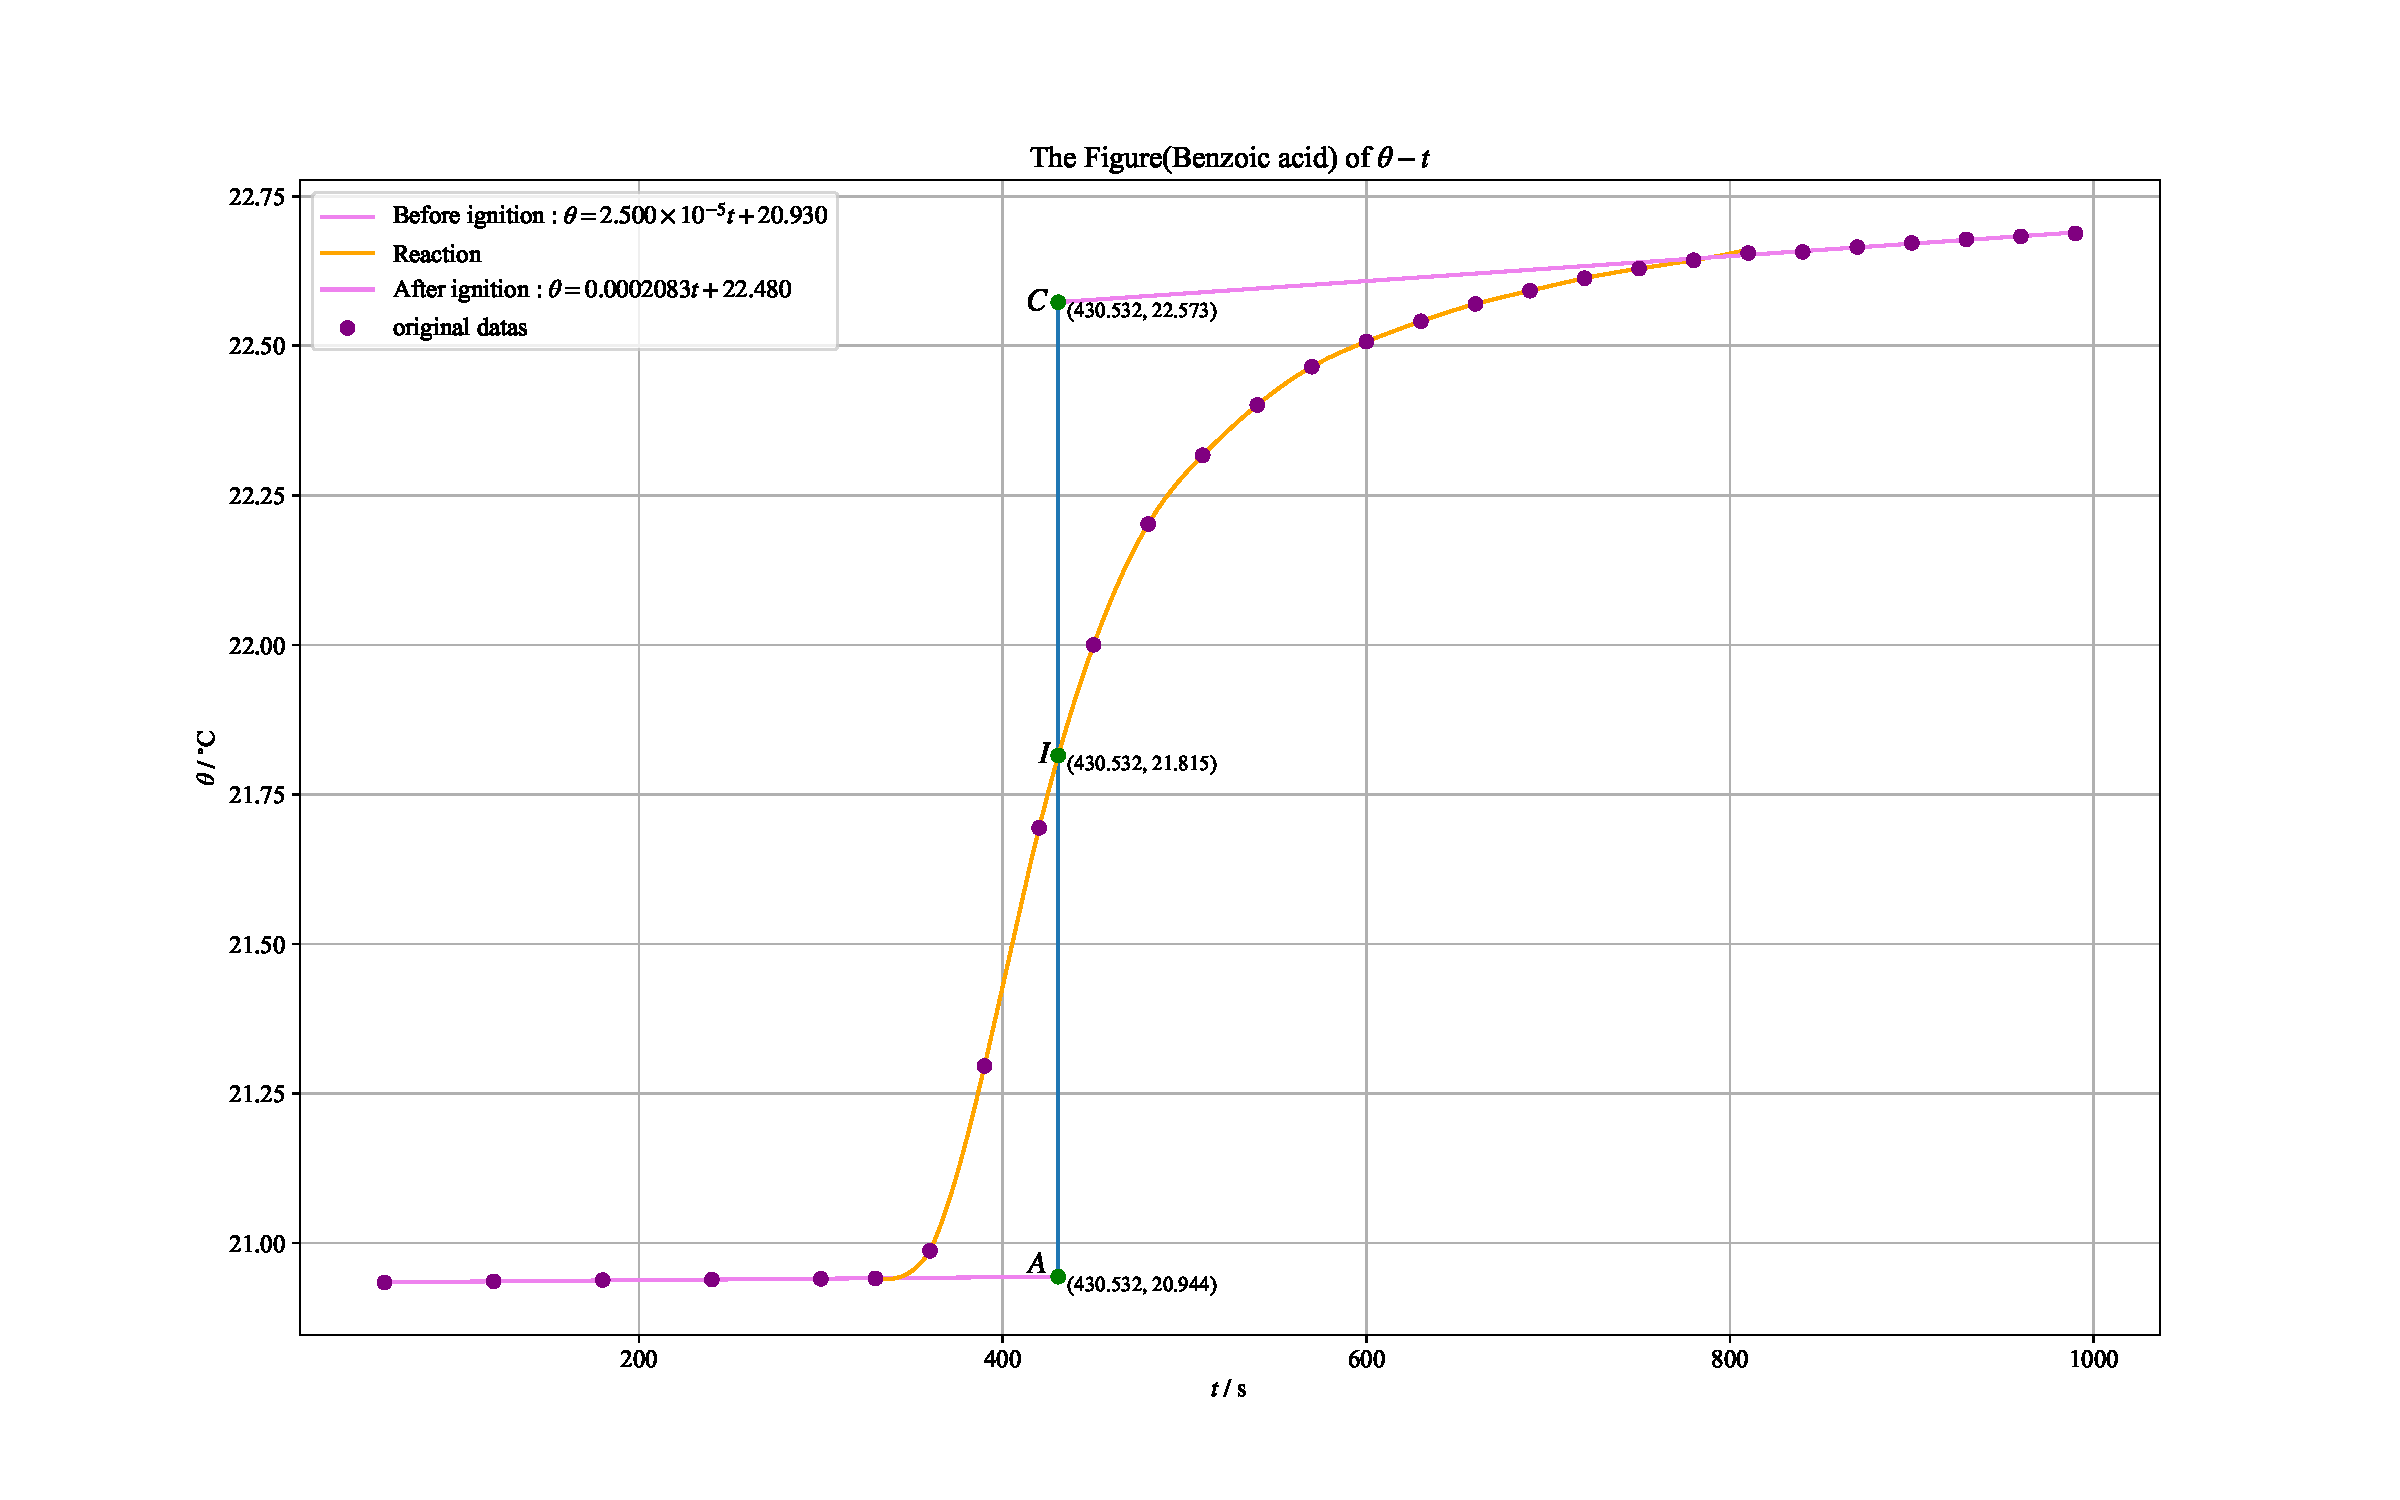
\includegraphics[scale=0.4]{Fig2}
	\caption{苯甲酸的雷诺校正曲线。纵坐标$\theta$为温度(去单位为摄氏度$^{\circ}$C),横坐标$t$为时间(去单位为 秒 s),$C$点与$A$点纵坐标差值为升高温度为$1.629^{\circ}$C}
	\label{fi8}
\end{figure}

\newpage
\begin{table}[h]
		\centering
		\begin{tabular}{p{3cm}<{\centering} p{3cm}<{\centering} p{3cm}<{\centering} p{3cm}<{\centering}}
		\toprule
		\multicolumn{2}{c}{蔗糖} &   \multicolumn{2}{c}{苯甲酸}   \\  
		\midrule
        时间$t$/s & 温差$\Delta\theta/^{\circ}$C & 时间$t$/s & 温差$\Delta\theta/^{\circ}$C \\  
        \midrule
        0 & 0.000 & 0 & 0.000 \\  
        60 & 0.009 & 60 & 0.002 \\  
        120 & 0.016 & 120 & 0.004 \\  
        180 & 0.019 & 180 & 0.006 \\  
        240 & 0.023 & 240 & 0.007 \\  
        300 & 0.027 & 300 & 0.008 \\  
        330 & 0.029 & 330 & 0.009 \\ 
        \rowcolor{mypink} 
        360 & 0.129 & 360 & 0.055 \\  
        390 & 0.477 & 390 & 0.364 \\  
        420 & 0.693 & 420 & 0.762 \\  
        450 & 0.821 & 450 & 1.068 \\  
        480 & 0.902 & 480 & 1.270 \\  
        510 & 0.960 & 510 & 1.385 \\  
        540 & 1.002 & 540 & 1.469 \\  
        570 & 1.027 & 570 & 1.533 \\  
        600 & 1.053 & 600 & 1.575 \\  
        630 & 1.075 & 630 & 1.609 \\  
        660 & 1.094 & 660 & 1.638 \\  
        690 & 1.110 & 690 & 1.660 \\  
        720 & 1.122 & 720 & 1.681 \\  
        750 & 1.134 & 750 & 1.697 \\  
        780 & 1.146 & 780 & 1.711 \\  
        810 & 1.550 & 810 & 1.723 \\
        \rowcolor{mycyan}  
        840 & 1.163 & 840 & 1.725 \\  
        870 & 1.172 & 870 & 1.733 \\  
        900 & 1.178 & 900 & 1.740 \\  
        930 & 1.185 & 930 & 1.746 \\  
        960 & 1.191 & 960 & 1.751 \\  
         & &990 & 1.756   \\  
		\bottomrule
		\end{tabular}	
		\label{ta1}
		\caption{实验数据(标有\textcolor{mypink}{粉色},是点火;标有\textcolor{mycyan}{蓝色},是结束反应)}
\end{table}
\newpage
	\section{实验二:蔗糖水解}
	
	\begin{figure}[h]
	\centering
	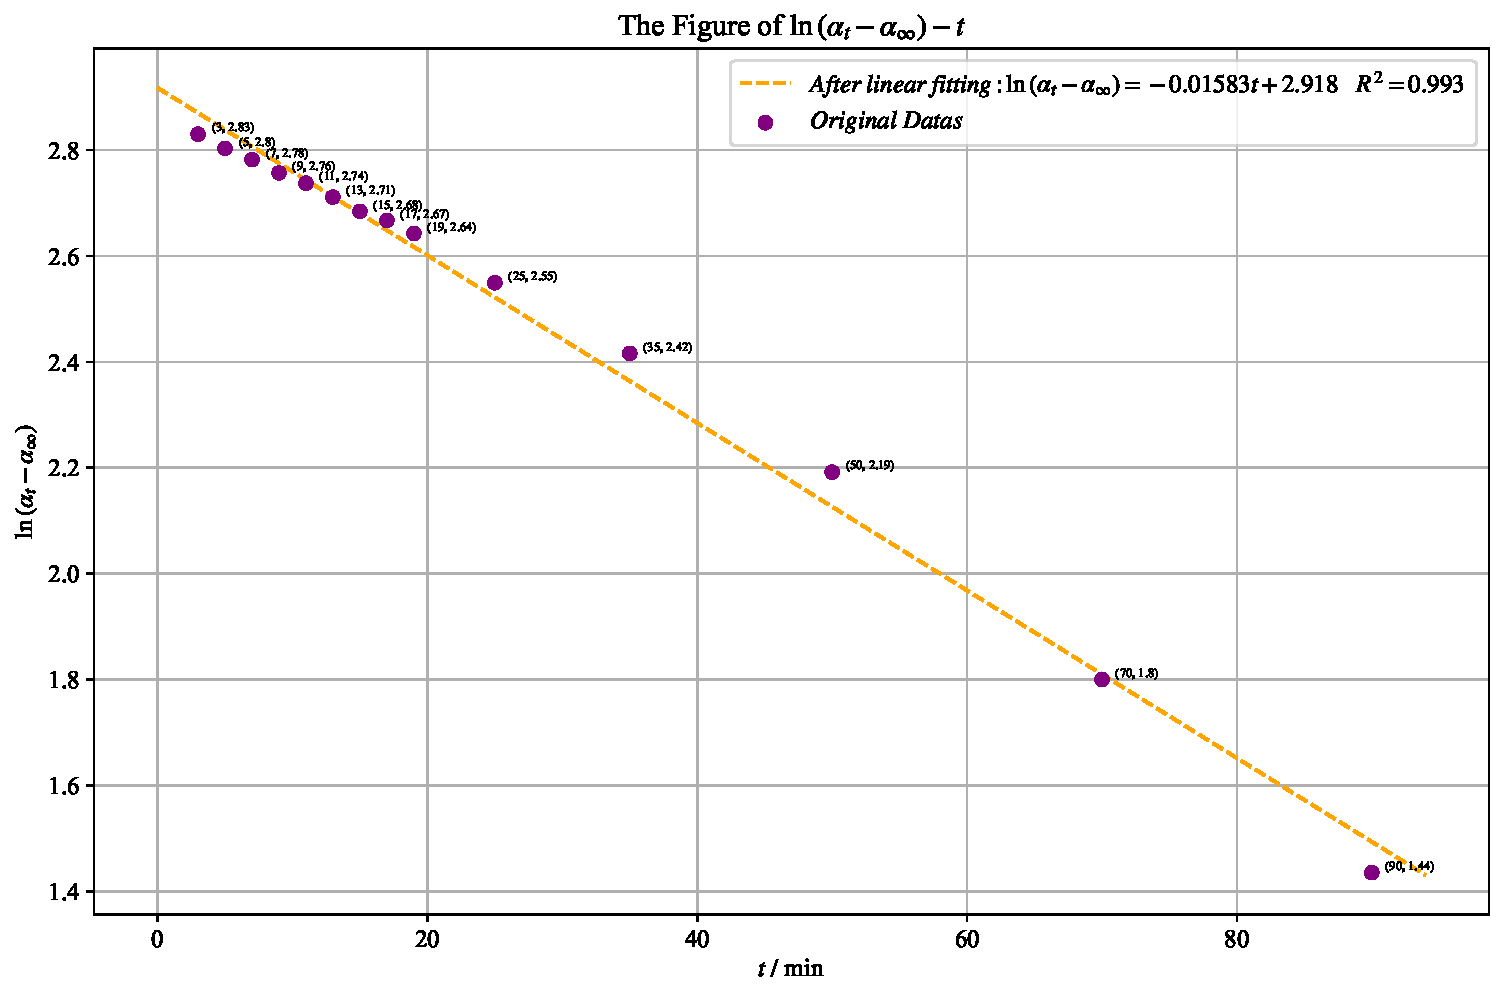
\includegraphics[scale=0.5]{ffigg}
	\caption{$\ln{(\alpha_{t}-\alpha_{\infty})}$对时间$t$(去除单位为 min)作图,得到直线的表达式为\textcolor[rgb]{0.54,0.13,0.33}{$\ln{(\alpha_{t}-\alpha_{\infty})} = -0.01621t+2.91$},应满足形式\ \textcolor[rgb]{0.07,0.36,0.57}{$\ln{(\alpha_{t}-\alpha_{\infty})} = -kt+\ln{(\alpha_{0}-\alpha_{\infty})}$}。拟合曲线对应的斜率为\textcolor[rgb]{0.54,0.13,0.33}{$-0.01621$},其相反数即为反应速率常数\textcolor[rgb]{0.54,0.13,0.33}{$k = 0.01621$}。}
	\label{fi3}
\end{figure}
\setlength{\tabcolsep}{1mm}{
\begin{table}[!ht]
		\centering
		\begin{tabular}{ccccccccccccccc}
 \toprule
  时间\textcolor[rgb]{0.54,0.13,0.33}{$t$}/min & 3 & 5 & 7 & 9 & 11 & 13 & 15 & 17 & 19 & 25 & 35 & 50 & 70 & 90 \\ 
   \midrule
       $a_{t}'$(原始数据) & 12.15 & 11.70 & 11.35 & 10.95 & 10.65 & 10.25 & 9.85 & 9.60 & 9.25 & 8.00 & 6.40 & 4.15 & 1.25 & -0.60 \\
       
       $a_{t}$(修正数据) & 12.35& 11.90 & 11.55& 11.15 &10.85& 10.45 &10.05 & 9.80  & 9.45 & 8.20 &  6.60  & 4.35&  1.45& -0.40\\
       
        $a_{t} - a_{\infty}$ &16.95 &16.50 & 16.15 &15.75 &15.45 &15.05 &14.65 &14.40&  14.05& 12.80&  11.20 &  8.95  & 6.05  &4.20 \\ 
        
        \textcolor[rgb]{0.54,0.13,0.33}{$\ln{(a_{t}-a_{\infty})}$}& 2.83 & 2.80& 2.78& 2.76& 2.74&   2.71 & 2.68& 2.67 & 2.64 &  2.55 & 2.42 & 2.19 &  1.80 & 1.44 \\ \midrule
        \multicolumn{15}{c}{$a_{\infty} = -4.60$}\\
 \bottomrule
		\end{tabular}	
		\label{ta2}
		\caption{实验数据计算整理}
\end{table}
}

	
	\section{}
	\section{}
	\section{}
	
	\section{实验六:原电池电动势的测定}
	\begin{figure}[h]
	\centering
	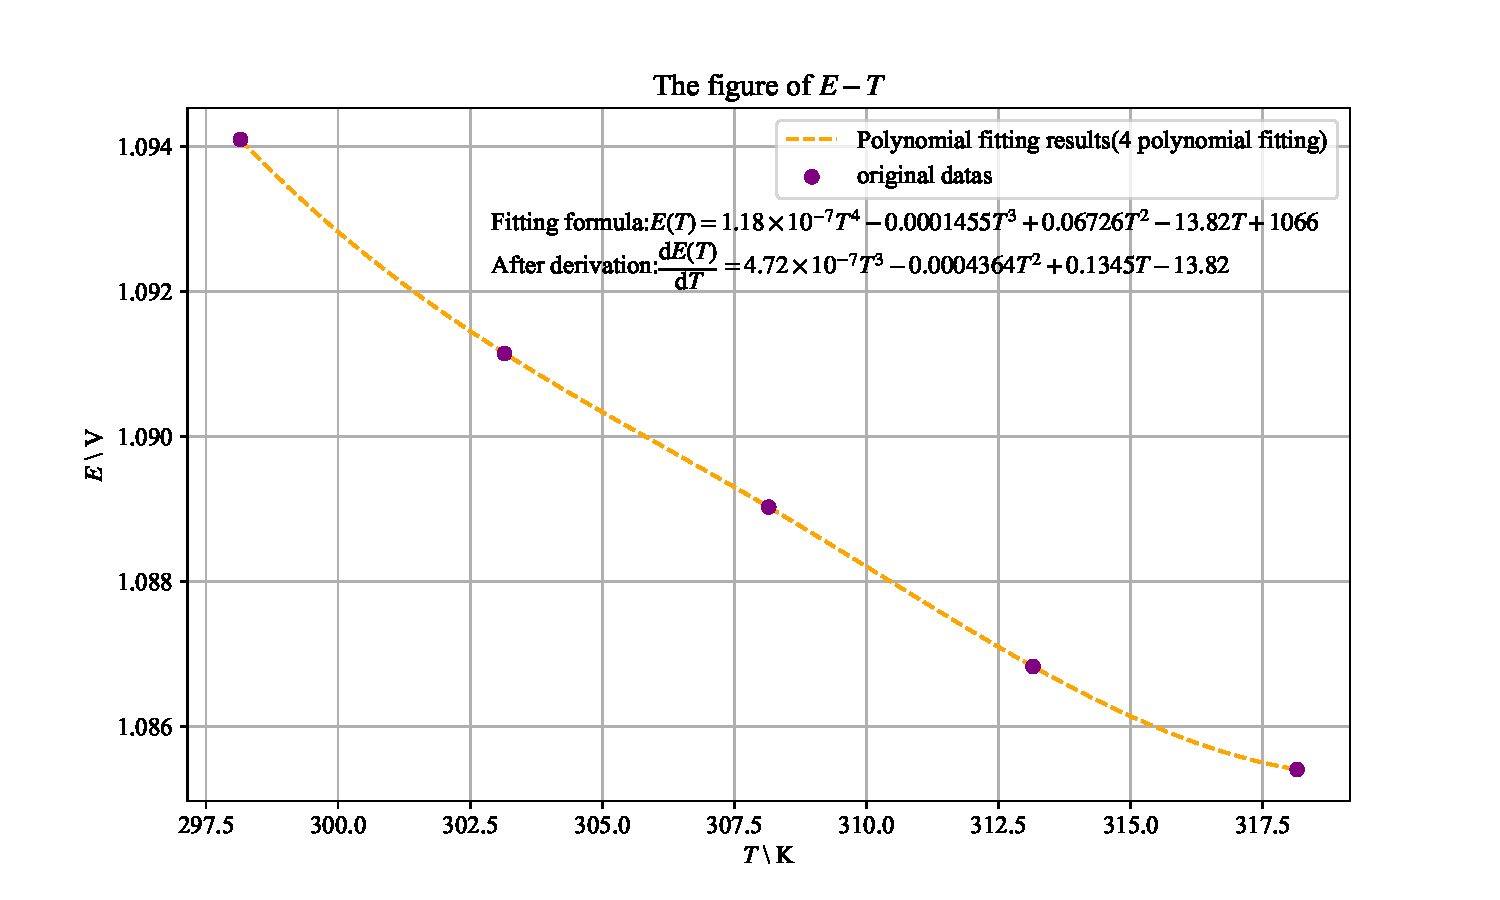
\includegraphics[scale=0.63]{6}
	\caption{利用四次多项式拟合得到的$E-T$曲线,其中横坐标为热力学温度$T$(单位:开尔文 K),纵坐标为原电池$\ce{Zn}_{(\rm{s}})|\ce{ZnSO4}(0.1\rm{mol}/L)||\ce{CuSO4}(0.1\rm{mol/L})|\ce{Cu}_{(\rm{s})}$的电池电动势 $E$(单位:伏特 V)。多项式拟合结果为:\textcolor[rgb]{0.54,0.13,0.33}{$E(T) =1.18\times 10^{-7} T^{4} - 0.0001455 T^{3} + 0.06726 T^{2} - 13.82 T + 1066$},公式中的 $E(T)$与$T$视作无量纲数,即:$E(T) = \dfrac{E(T)}{\ce{V}}$,$T = \dfrac{T}{\ce{K}}$,上式两边对温度$T$求一阶导数,$E(T)$恒压下为温度$T$的函数,得:\textcolor[rgb]{0.54,0.13,0.33}{$\pqty{\dfrac{\partial E}{\partial T}}_{p} = \dfrac{{\rm{d}}E(T)}{{\rm{d}}T} = 4.72\times 10^{-7} T^{3} - 0.0004364 T^{2} + 0.1345 T - 13.82$}。}
	\label{fi1}
\end{figure}
\newpage
\section{实验七:溶液表面张力的测定}
\begin{figure}[h]
	\centering
	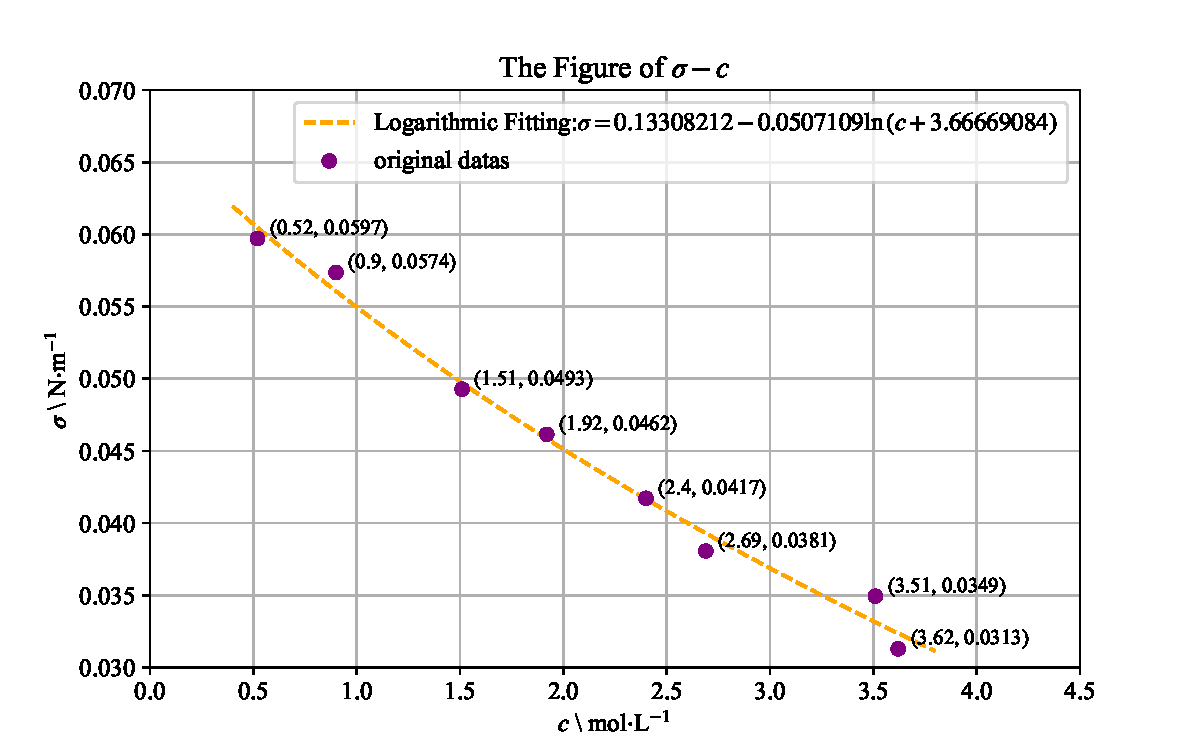
\includegraphics[scale=0.8]{Figure1}
	\caption{利用函数$\sigma = a + b \ln{(c + d)}$拟合得到的$\sigma - c$曲线。其中$a,b,d$均为参数,$c$为乙醇溶液的浓度(去除单位为:mol$\cdot$m$^{-1}$),$\sigma$为溶液表面张力(去除单位为:N$\cdot$m$^{-2}$)得到的拟合拟合结果为:\textcolor[rgb]{0.54,0.13,0.33}{$ \sigma= 0.13308212+0.0507109\ln{(c + 3.66669084)}$},回归系数$R^{2} = 0.993$。}
	\label{fi2}
\end{figure}
\newpage
\begin{figure}[h]
	\centering
	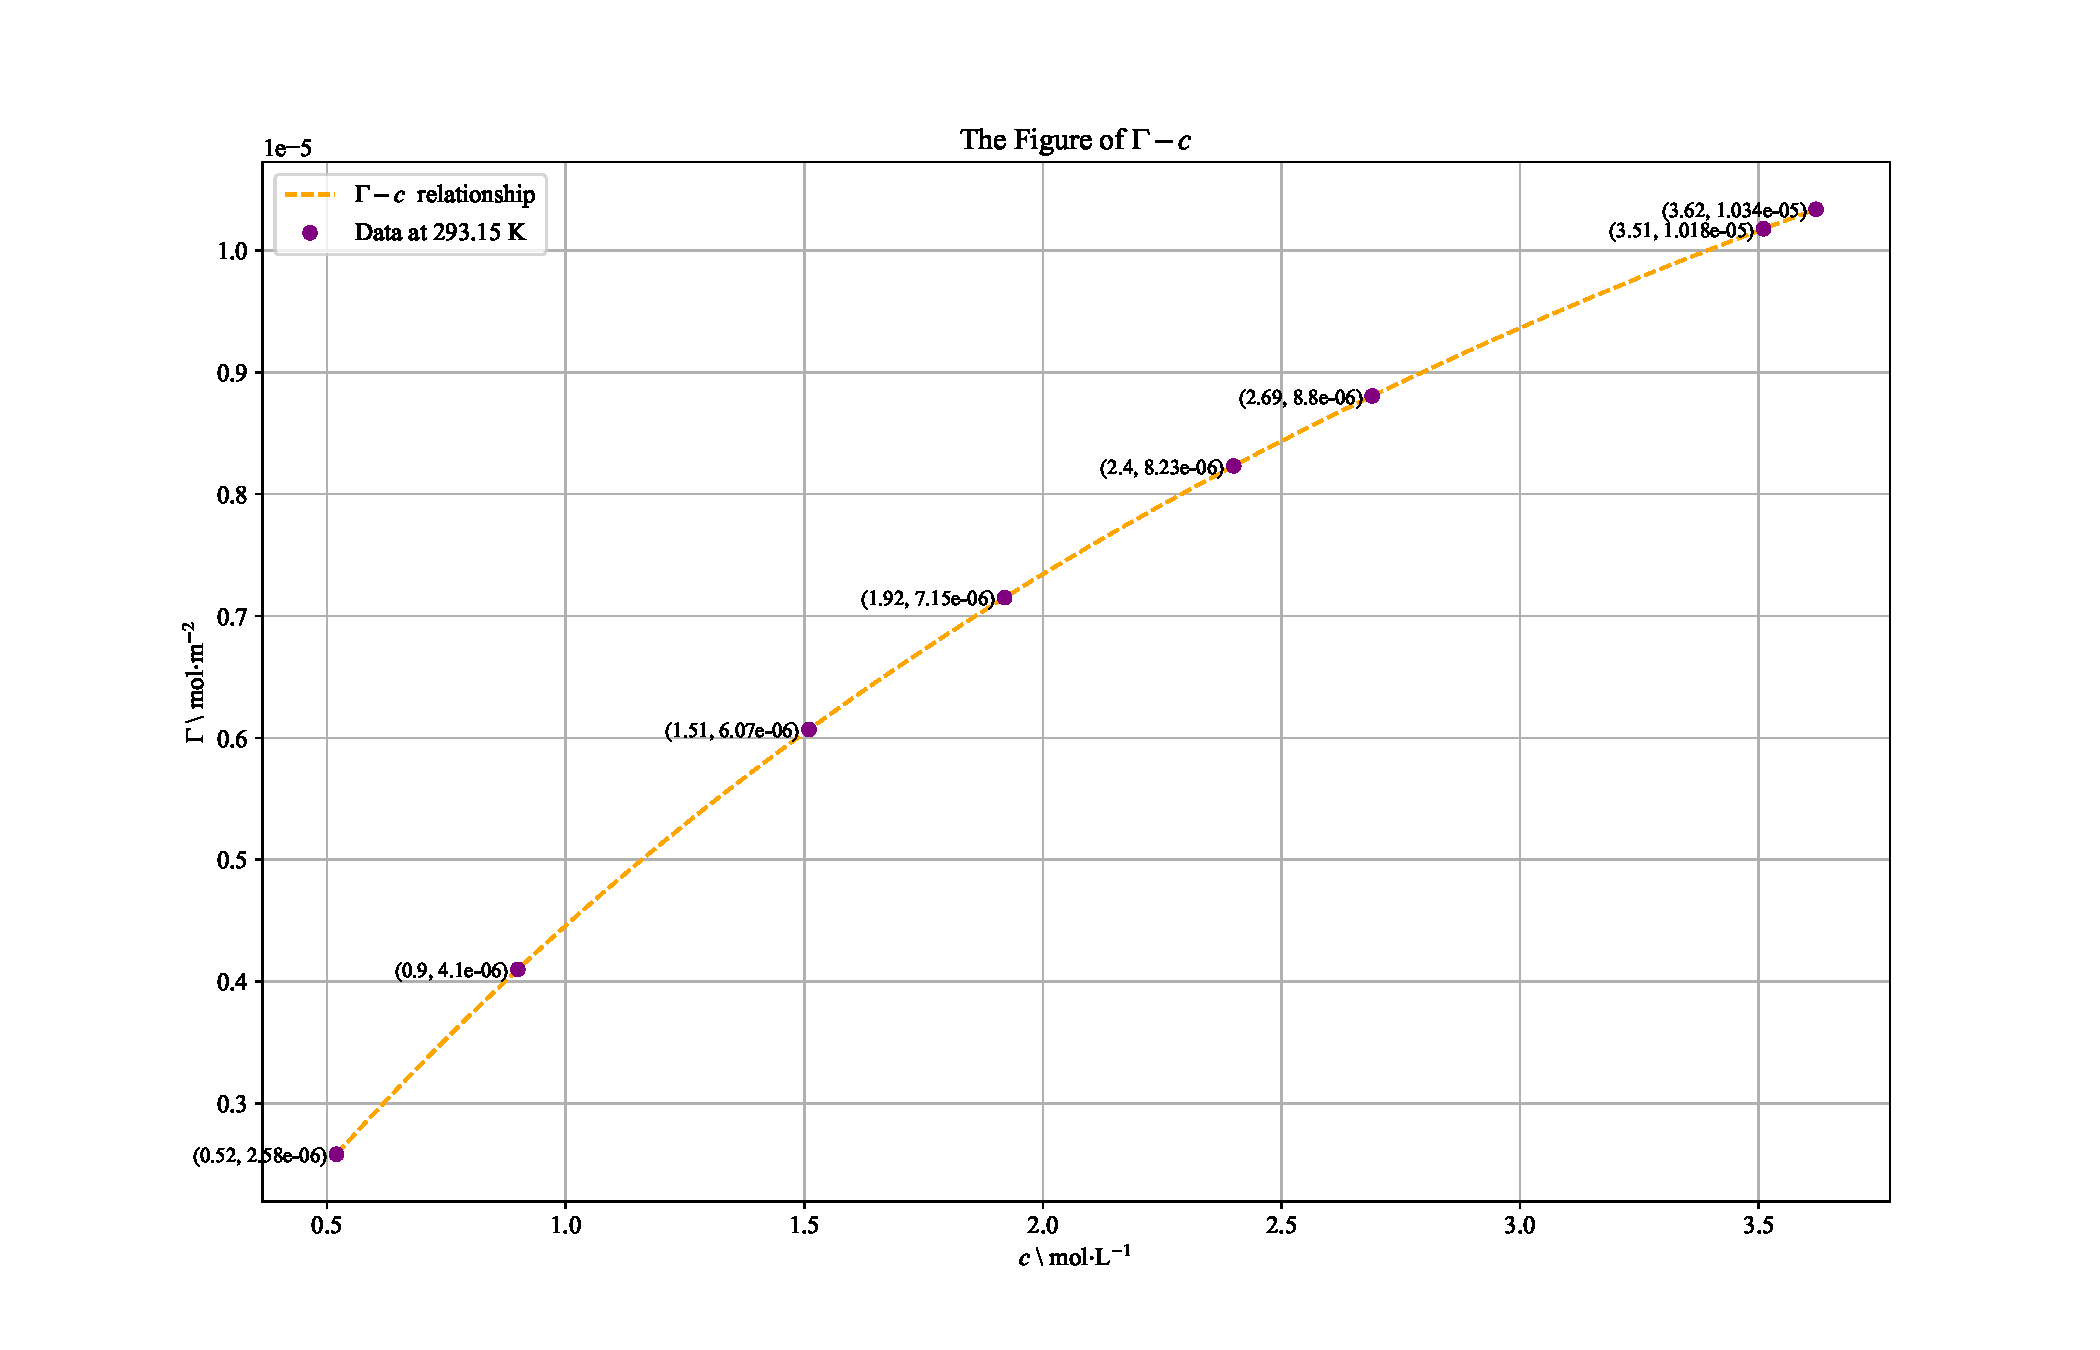
\includegraphics[scale=0.8]{Figure2}
	\caption{利用$\sigma - c$的拟合结果求出$\varGamma - c$曲线。其中$\varGamma$是溶质在表面层的吸附量(去除单位为 mol$\cdot$ m$^{-2}$,纵坐标为$1\times 10^{-5}$mol$\cdot$ m$^{-2}$),计算公式为\textcolor[rgb]{0.07,0.36,0.57}{$\varGamma = \dfrac{c}{RT}\pqty{\dfrac{\rm{d}\sigma}{\rm{d}c}}_{T}$},其中 $T$取实验温度$T = 293.15$K。}
	\label{fi3}
\end{figure}

\begin{figure}[h]
	\centering
	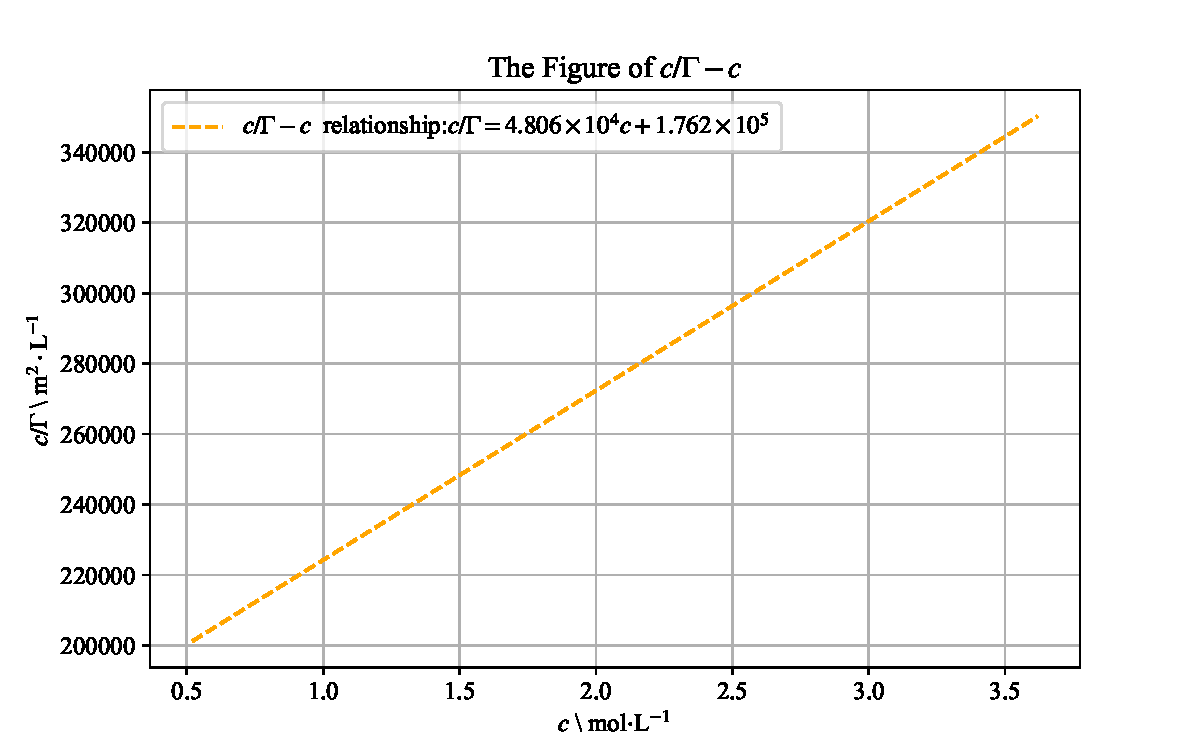
\includegraphics[scale=0.8]{Figure3}
	\caption{$\dfrac{c}{\varGamma}-c$关系图,纵坐标为$\dfrac{c}{\varGamma}$(去单位为m$^{-1}$),横坐标为$c$(去单位为 mol$\cdot $m$^{-3}$)。利用一次拟合,得到一直线,关系式为\textcolor[rgb]{0.54,0.13,0.33}{$\dfrac{c}{\varGamma} = 4.806 \times 10^{4}c + 1.762 \times 10^{8}$},应符合关系式\textcolor[rgb]{0.07,0.36,0.57}{$\dfrac{c}{\varGamma} = \dfrac{c}{\varGamma_{\infty}}+\dfrac{1}{K\varGamma_{\infty}}$},故其斜率之倒数为$\varGamma_{\infty} = 2.081 \times10^{-5}$mol$\cdot$ m$^{-2}$}
	\label{fi4}
\end{figure}
\newpage
\section{实验八:弱电解质电离平衡常数的测定}
\begin{figure}[h]
	\centering
	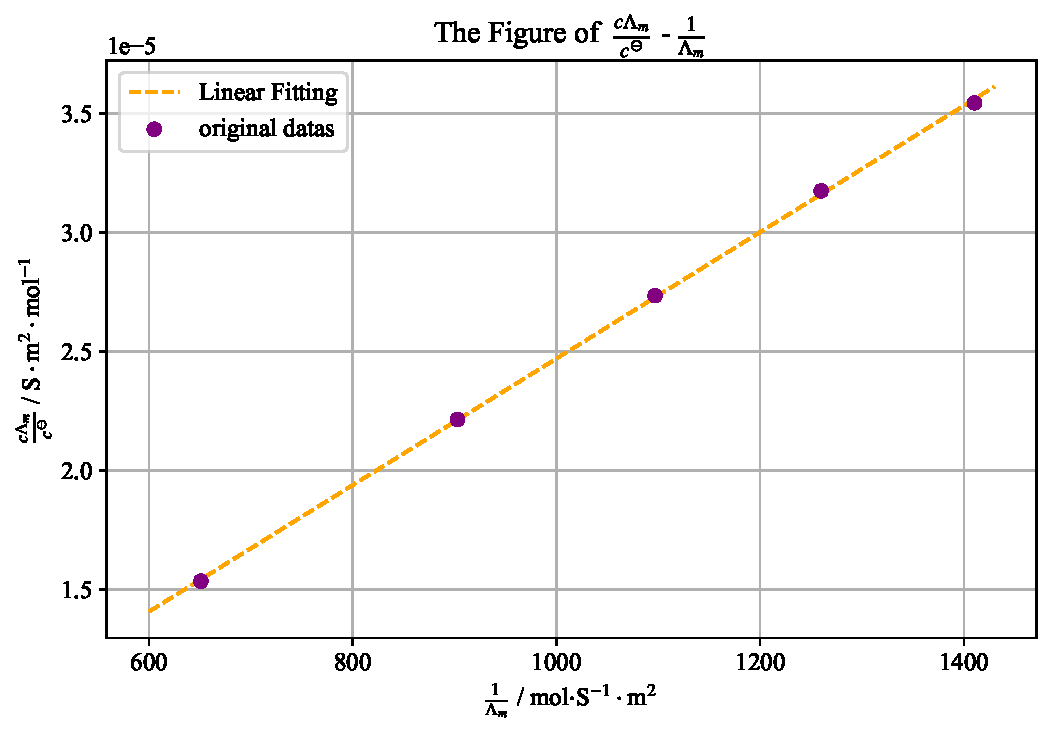
\includegraphics[scale=0.8]{Map}
	\caption{$\dfrac{c\varLambda_{m}}{c^{\ominus}} $(去单位为$\rm{S}\cdot\rm{m}^{2}\cdot\rm{mol}^{-1}$)对$ \dfrac{1}{\varLambda_{m}}$(去单位为$\rm{mol}\cdot\rm{S}^{-1}\cdot\rm{m}^{-2}$)作图,得到的方程为\textcolor[rgb]{0.54,0.13,0.33}{$\dfrac{c\varLambda_{m}}{c^{\ominus}} =2.657\times 10^{-8} \dfrac{1}{\varLambda_{m}}- 1.867\times 10^{-6}$},用斜率除以$\varLambda_{m,\infty}^{2}$,就得到\textcolor[rgb]{0.54,0.13,0.33}{$K_{c}^{\ominus} = 1.741\times 10^{-5}$}。}
	\label{fi5}
\end{figure}


\end{document}
